% chapters/08-technology-operations.tex

\chapter{Technology and Operations}

\begin{importantbox}
This chapter provides comprehensive guidance on setting up your technology infrastructure and operations in Nigeria, with specific considerations for different business types and regions.
\end{importantbox}

\FloatBarrier
\section{Digital Infrastructure Setup}

\subsection{Core Technology Stack}
\begin{figure}[htbp]
    \centering
    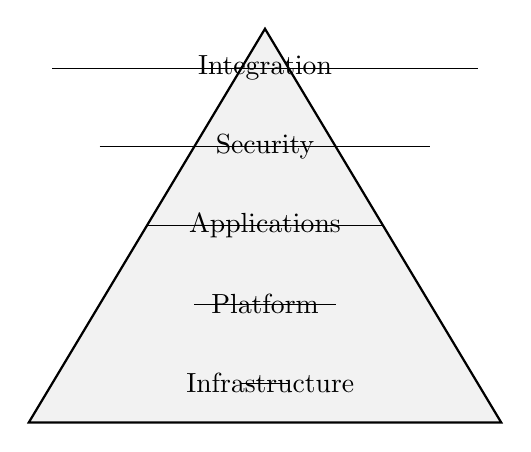
\begin{tikzpicture}[
        layer/.style={text width=2cm, align=center}
    ]
        % Technology stack pyramid with better proportions
        \fill[gray!10] (0,0) -- (6,0) -- (3,5) -- cycle;

        % Horizontal layers with better spacing
        \foreach \y/\label in {
            0.5/Infrastructure,
            1.5/Platform,
            2.5/Applications,
            3.5/Security,
            4.5/Integration
        } {
            \pgfmathsetmacro{\width}{6-\y*1.2}
            \draw (\width/2,\y) -- (6-\width/2,\y);
            \node[layer] at (3,\y) {\label};
        }

        % Outer pyramid
        \draw[thick] (0,0) -- (6,0) -- (3,5) -- cycle;
    \end{tikzpicture}
    \caption{Technology Stack Components}
    \label{fig:tech-stack}
\end{figure}

\subsection{Infrastructure Requirements Matrix}
\begin{center}
\begin{tabularx}{\textwidth}{>{\raggedright\arraybackslash}X >{\raggedright\arraybackslash}X >{\raggedright\arraybackslash}X >{\raggedright\arraybackslash}X}
    \toprule
    \textbf{Component} & \textbf{Basic} & \textbf{Advanced} & \textbf{Enterprise} \\
    \midrule
    Servers & Cloud-based & Hybrid & Multi-region \\
    Storage & Standard & Redundant & Distributed \\
    Network & Broadband & Dedicated & Multi-carrier \\
    Security & Essential & Enhanced & Comprehensive \\
    \bottomrule
\end{tabularx}
\end{center}

\section{Operations Management Framework}

\subsection{Core Operational Processes}
\begin{tcolorbox}[colback=white,colframe=primarydark,title=\textbf{Process Categories}]
\begin{itemize}
    \item Core Business Processes
    \item Support Functions
    \item Management Systems
    \item Quality Control
    \item Performance Monitoring
\end{itemize}
\end{tcolorbox}

\FloatBarrier
\section{Regional Technology Considerations}

% UK Region
\begin{regionalbox}{United Kingdom}
\textbf{Financial Services Systems}
\begin{itemize}
    \item Payment processing platforms
    \item Regulatory reporting systems
    \item Compliance monitoring tools
    \item Data protection infrastructure
\end{itemize}
\end{regionalbox}

\subsection{UK FinTech Architecture}
\begin{figure}[htbp]
    \centering
    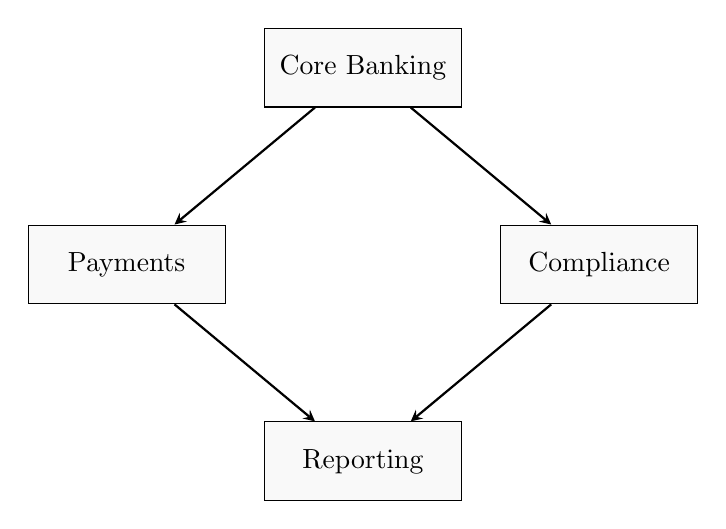
\begin{tikzpicture}[
        node distance=2.5cm,
        box/.style={draw, minimum width=2.5cm, minimum height=1cm, align=center, fill=gray!5},
        arrow/.style={-stealth, thick}
    ]
        % Financial systems architecture with improved layout
        \node[box] (core) at (0,0) {Core Banking};
        \node[box] (payment) at (-3,-2.5) {Payments};
        \node[box] (compliance) at (3,-2.5) {Compliance};
        \node[box] (reporting) at (0,-5) {Reporting};

        % Connect components with styled arrows
        \draw[arrow] (core) -- (payment);
        \draw[arrow] (core) -- (compliance);
        \draw[arrow] (payment) -- (reporting);
        \draw[arrow] (compliance) -- (reporting);
    \end{tikzpicture}
    \caption{Financial Services System Architecture}
    \label{fig:fintech-arch}
\end{figure}

% US Region
\begin{regionalbox}{United States}
\textbf{Tech Platform Integration}
\begin{itemize}
    \item Cloud infrastructure
    \item Development environments
    \item API integration
    \item Scalability framework
\end{itemize}
\end{regionalbox}

\subsection{US Tech Stack Implementation}
\begin{center}
\begin{tabularx}{\textwidth}{>{\raggedright\arraybackslash}X >{\raggedright\arraybackslash}X >{\raggedright\arraybackslash}X}
    \toprule
    \textbf{Layer} & \textbf{Components} & \textbf{Integration} \\
    \midrule
    Frontend & User Interface & API Gateway \\
    Backend & Business Logic & Microservices \\
    Database & Data Storage & Replication \\
    \bottomrule
\end{tabularx}
\end{center}

% UAE Region
\begin{regionalbox}{UAE}
\textbf{Trade and Logistics Systems}
\begin{itemize}
    \item Inventory management
    \item Supply chain tracking
    \item Customs documentation
    \item Logistics coordination
\end{itemize}

\subsection{UAE Trade Systems Architecture}
\begin{tcolorbox}[colback=white,colframe=primary,title=\textbf{System Components}]
\begin{enumerate}
    \item Order Management System
    \item Warehouse Management System
    \item Transportation Management System
    \item Documentation Management System
    \item Customs Interface
\end{enumerate}
\end{tcolorbox}
\end{regionalbox}

% Canada Region
\begin{regionalbox}{Canada}
\textbf{Industry-Specific Solutions}
\begin{itemize}
    \item Agricultural monitoring
    \item Environmental tracking
    \item Quality assurance systems
    \item Compliance monitoring
\end{itemize}

\subsection{Canadian Industry Solutions}
\begin{center}
\begin{tabularx}{\textwidth}{>{\raggedright\arraybackslash}X >{\raggedright\arraybackslash}X >{\raggedright\arraybackslash}X}
    \toprule
    \textbf{Industry} & \textbf{Core Systems} & \textbf{Integration Points} \\
    \midrule
    Agriculture & Field Management & Supply Chain \\
    Environment & Monitoring Tools & Reporting \\
    Manufacturing & Production Control & Quality Assurance \\
    \bottomrule
\end{tabularx}
\end{center}
\end{regionalbox}

\FloatBarrier
\section{Quality Control Systems}

\subsection{Quality Management Framework}
\begin{figure}[htbp]
    \centering
    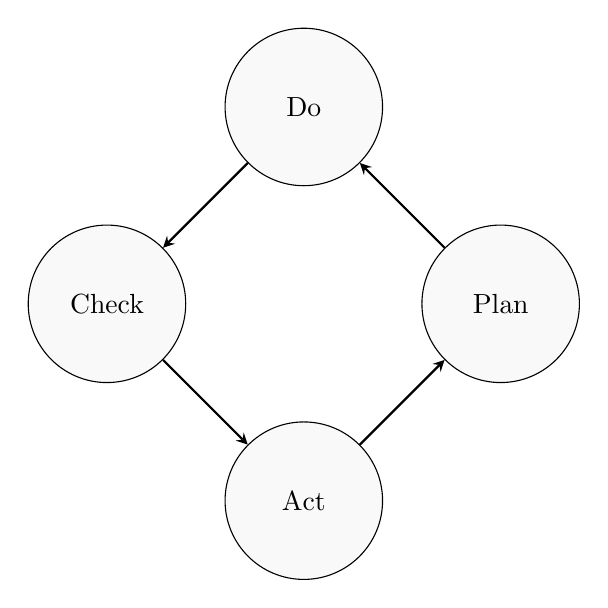
\begin{tikzpicture}[
        node distance=3cm,
        phase/.style={draw, circle, minimum size=2cm, text width=1.5cm, align=center, fill=gray!5},
        arrow/.style={-stealth, thick, bend left=15}
    ]
        % Quality management cycle with improved styling
        \foreach \angle/\label in {
            0/Plan,
            90/Do,
            180/Check,
            270/Act
        } {
            \node[phase] (phase-\angle) at (\angle:2.5) {\label};
        }

        % Connect phases with curved arrows
        \draw[arrow] (phase-0) -- (phase-90);
        \draw[arrow] (phase-90) -- (phase-180);
        \draw[arrow] (phase-180) -- (phase-270);
        \draw[arrow] (phase-270) -- (phase-0);
    \end{tikzpicture}
    \caption{Quality Management Cycle}
    \label{fig:quality-cycle}
\end{figure}

\section{Performance Monitoring}

\subsection{KPI Dashboard Framework}
\begin{tcolorbox}[colback=white,colframe=primarydark,title=\textbf{Key Performance Indicators}]
\begin{itemize}
    \item Operational Efficiency
    \item System Uptime
    \item Process Compliance
    \item Error Rates
    \item Response Times
\end{itemize}
\end{tcolorbox}

\begin{communitybox}
Access technology and operations resources on the Africa Growth Circle:
\begin{itemize}
    \item System setup guides
    \item Vendor recommendations
    \item Implementation templates
    \item Tech support network
    \item Operations best practices
\end{itemize}
Visit circle.counseal.com for technology support.
\end{communitybox}

\begin{workshopbox}
\textbf{Chapter 8 Technology Planning Workshop}

1. Infrastructure Planning
\begin{itemize}
    \item Core systems needed: \_\_\_\_\_\_\_\_\_
    \item Integration requirements: \_\_\_\_\_\_\_\_\_
    \item Security considerations: \_\_\_\_\_\_\_\_\_
\end{itemize}

2. Operations Setup
\begin{itemize}
    \item Process documentation: \_\_\_\_\_\_\_\_\_
    \item Quality controls: \_\_\_\_\_\_\_\_\_
    \item Performance metrics: \_\_\_\_\_\_\_\_\_
\end{itemize}

3. Implementation Timeline
\begin{itemize}
    \item System selection: \_\_\_\_\_\_\_\_\_
    \item Setup phases: \_\_\_\_\_\_\_\_\_
    \item Testing schedule: \_\_\_\_\_\_\_\_\_
\end{itemize}

Download technical implementation guides from the Africa Growth Circle platform.
\end{workshopbox}

\begin{importantbox}
In Chapter 9, we'll explore strategies for growth and scaling your operations once your technology infrastructure is in place.
\end{importantbox}